\chapter{The writing system}

\epigraph{What remains\\
is not what was there\\
but what persisted.}{}

Chapter \ref{ch:vocabulary} dealt with language at the word level, and Chapter \ref{ch:sound} dealt with the syllable and phoneme levels. These levels are progressively less accessible to our conscious attention. Most pre-literate English-speaking children have no trouble identifying and counting words (assuming they can count). Syllables are less natural and take a little bit of practice. It helps to sing and clap along. 

Phonemes, on the other hand, are deeply inaccessible to our conscious awareness. No pre-literate child could tell you that \textit{cat} has three ``sounds'' or that \textit{jump} has four. In fact, it seems that there is a reciprocal causal relationship between learning to read an alphabet like the one English uses and \textsc{phonemic awareness}: you can't develop it without exposure to an alphabet and you can't successfully learn to read an alphabet without phonemic awareness.

But not all writing is alphabetic, and not all writing systems require phonemic awareness, meaning that some students may arrive in your class with un- or underdeveloped phonemic awareness.

\section{Writing systems}
Simplifying somewhat, we can say that there are three major types of writing systems in the world. The first is logographic. Chinese is an example of a logographic writing system. The word for `outside' in Mandarin is \textit{wài}, and it's written ⟨外⟩. The character ⟨外⟩ doesn't represent the phonemes or the syllable. Instead, it represents a whole word. In Cantonese, this same character represents \textit{ngoi}, while still meaning `outside'.

If this seems a little mysterious, it may be easier to understand the concept with the Arabic numerals, which are also logographic. For instance \textit{7}, as in \textit{7:00}, doesn't encode the phonemes /sɛvən/. Nor does it encode the syllables se-ven. \textit{7} represents a whole word, as do ⟨3⟩ in \textit{\$3} or ⟨0⟩ in \textit{0 degrees}. But while it's \textit{seven} for an English speaker, it's \textit{efta} for a Greek speaker and \textit{saba} in Swahili.

Logographic systems like these are the easiest to learn in terms of individual characters. All you have to do is associate the word with a character. They have the drawback, though, of typically having thousands of characters to learn.

The next easiest system is syllabic. A good example is the Japanese kana. Remember that consonant clusters are not possible in Japanese, so McDonald's is pronounced with a bunch of extra vowels as /ma.ku.do.na.ru.do/. Each CV there is a syllable and each one has its own character: ⟨マクドナルド⟩. Such systems are also relatively easy to learn because syllabic awareness is fairly easy to develop. If you have a limited syllable inventory, as Japanese does, then there aren't even that many characters to learn. English, though, has thousands of syllables, so this makes syllabic writing a poor choice for us.

You're, of course, familiar with the English alphabet, which is based on the Roman alphabet. You may not realize that \textit{alphabet} does not denote the specific set of symbols you're reading right now. Russian is written in the Russian Cyrillic alphabet ⟨русский⟩, and Kurdish in the Kurdish Arabic alphabet ⟨کوردی⟩.

What distinguishes alphabets from other writing systems is that they (primarily) represent individual phonemes. They do this better in some languages, like Finnish and Greek, and worse in others like English and French. Finnish has more or less a one-to-one relationship between letters and phonemes, making it extremely easy to learn to decode Finnish words. English, sadly, has a many-to-many relationship, even if you ignore allophones (Section \ref{sec:allophones}). 

Multiple graphemes may represent the same phoneme:

\begin{itemize}[noitemsep]
    \item /f/ can be spelled as ⟨f⟩ \textit{\uline{f}ar}, ⟨ph⟩ \textit{\uline{ph}one}, or ⟨gh⟩ \textit{enou\uline{gh}}.
    \item /k/ can be ⟨c⟩ \textit{\uline{c}at}, ⟨k⟩ \textit{\uline{k}ite}, ⟨ck⟩ \textit{ba\uline{ck}}, ⟨ch⟩ \textit{\uline{ch}orus}, or ⟨que⟩ \textit{uni\uline{que}}.
\end{itemize}
        
Conversely, a single grapheme may represent multiple phonemes:
\begin{itemize}[noitemsep]
    \item ⟨c⟩ can represent /s/ as in \textit{\uline{c}ity}, or /k/ as in \textit{\uline{c}at}.
    \item ⟨g⟩ can represent /g/ as in \textit{\uline{g}o}, or /d͡ʒ/ as in \textit{\uline{g}iant}.
\end{itemize}
        
And, of course, there are various silent letters.

\begin{itemize}[noitemsep]
    \item ⟨k⟩ is silent in \textit{\uline{k}night} and \textit{\uline{k}nife}, pronounced /nʌɪt/ and /nʌɪf/ respectively.
    \item ⟨w⟩ is silent in \textit{\uline{w}rite} and \textit{\uline{w}rong}, pronounced /rʌɪt/ and /rɒŋ/.
    \item ⟨b⟩ is silent in \textit{dou\uline{b}t} and \textit{su\uline{b}tle}, pronounced /daʊt/ and /sʌtəl/.
    \item ⟨h⟩ is silent in \textit{\uline{h}onest} and \textit{g\uline{h}ost}, pronounced /ɒnɪst/ and /ɡoʊst/.
    \item ⟨e⟩ is silent in \textit{cak\uline{e}} and \textit{bit\uline{e}}, making the vowels ``long'',\footnote{I'll note again that ``long'' vowels are not necessarily longer in duration than other vowels. See the discussion in Section \ref{sec:long-vowels}.} pronounced /keɪk/ and /baɪt/.
\end{itemize}

So, the very fact that English is alphabetic makes it difficult to learn \strong{if you haven't already learned to read an alphabet}, in other words, if you're illiterate or if you are literate only in a logographic or syllabic script. But very few people these days fall into those groups. Even Chinese speakers typically learn ``pinyin'' a way to write their language with the Roman alphabet. Beyond that, though, even if you come to English with phonemic awareness, the weak correspondences between spelling and pronunciation, between graphemes and phonemes, makes it much more difficult to learn to read and write than a language like Finnish, Italian, or Greek, where the correspondences are quite robust.

Reading well is so much more than being able to read words, but without being able to read words, no one can read well. One method that has proven very helpful in overcoming the kinds of word-reading difficulties faced by young children and some adults learning English is phonics.

\section{Phonics} \label{sec:phonics}

While writing systems provide the framework for representing language visually, teaching methods like phonics help bridge the gap between alphabetic written symbols and spoken language. \textsc{Phonics} is a method of teaching reading that focuses on the relationship between the sounds (phonemes) of spoken language and the letters (graphemes) used to represent those sounds in written language. It is a crucial component of early literacy instruction, as it helps learners develop the skills to decode unfamiliar words by sounding them out.

If you've learned to read through phonics or have taught your own children using this method, you're likely familiar with its basic principles and effectiveness for children. But it can also be a valuable way for adult English language learners to improve word reading skills, also known as decoding. When an adult struggles to read individual words in English, despite having adequate oral language proficiency, phonics instruction is often the most effective and efficient way to address this issue.

It's important to note that difficulty in reading individual words (\textsc{decoding}) is distinct from poor reading comprehension. While both can impact overall reading proficiency, comprehension issues are more likely to stem from a lack of vocabulary knowledge rather than decoding skills. But decoding is a prerequisite for comprehension; if a learner can't accurately read the words on the page, their understanding of the text as a whole will be compromised.

Phonics focuses on the relationship between the sounds (phonemes) of spoken language and the letters (graphemes) used to represent those sounds in written language. The goal of phonics instruction is to help learners develop the ability to decode unfamiliar words by applying their knowledge of letter--sound correspondences.

Unfortunately, as we've seen, the grapheme--phoneme correspondences can be unreliable, especially with vowels. A digraph like ⟨ea⟩, for instance, may be /i/ as in \textit{teach}, /iə/ as in \textit{real}, /ɛ/ as in \textit{head}, /e/ as in \textit{great}. Greater consistency can be achieved here by considering the vowel along with the coda, in other words the part of the word that's important for rhyming, often called the \textsc{rime}. For example, ⟨each⟩~is consistently /it͡ʃ/ whether the word be \textit{each}, \textit{teach}, \textit{reach}, \textit{beach}, \textit{peach}, or \textit{bleach}. Another example is ⟨ate⟩, which is quite consistently /eɪt/ in stressed syllables. (For a list of teachable grapheme--phoneme correspondences, see Section \ref{sec:gpcs-list}.)

It must be admitted that there are exceptions, such as \textit{water} for ⟨ate⟩~and \textit{treachery} for ⟨each⟩~, but the use of rimes as a spelling unit is generally more useful than focusing on individual vowel spellings.

The key principles and techniques of phonics include:

\begin{itemize}[noitemsep]
    \item Letter-sound correspondence: Learners are taught the most common correspondences (e.g., ⟨sh$\rangle=$~/ʃ/, ⟨ch$\rangle=$~/t͡ʃ/, ⟨th$\rangle=$~/θ/ or /ð/, ⟨ough$\rangle=$~/oʊ/, ⟨ate$\rangle=$~/eɪt/, etc.).
    \item Segmenting: Learners break words down into their syllables, rimes, and phonemes (e.g., \textit{attack}~=~/æ/~+~/tæk/, \textit{tack}~=~/t/~+~/æk/, \textit{ack}~=~/æ/~+~/k/).
    \item Blending: Learners practice combining syllables, rimes, and phonemes.
    \item Phoneme manipulation: Learners engage in activities that involve adding, deleting, or substituting syllables, rimes, and phonemes within words (e.g., changing \textit{cat} to \textit{hat} by replacing /k/ with /h/).
    \item Systematic progression: Phonics instruction typically follows a structured sequence, starting with simple, regular, high-frequency, correspondences and progressing to more complex, less regular, and less common patterns.
\end{itemize}

The goal is not to cover every possible grapheme--phoneme correspondence, but to get enough high-frequency ones that learners can start to work out the others.

Common materials used in phonics instruction include:

\begin{itemize}[noitemsep]
    \item Alphabet charts and flashcards: Visual aids that help learners associate letters with their corresponding sounds.
    \item Decodable texts: Books or passages that are carefully designed to feature words that can be sounded out using the letter-sound correspondences learned so far.
    \item Word lists and word families: Groups of words that share similar spelling patterns or rhymes, helping learners recognize common sound-spelling relationships.
    \item Manipulatives: Physical objects like letter tiles or magnetic letters that allow learners to actively engage with the process of blending and segmenting sounds.
    \item Multimedia resources: Digital tools, such as educational software or online games, that provide interactive practice with letter-sound correspondences and word decoding.
\end{itemize}

The ultimate goal of phonics instruction is to help learners become fluent and accurate readers who can independently decode unfamiliar words and comprehend written text. By developing a strong foundation in phonics, learners can recognize familiar words quickly and automatically, freeing up cognitive resources for comprehension. They can decode unfamiliar words by applying their knowledge of letter-sound relationships. And they can engage more confidently with a wide range of written texts, from basic instructions to complex academic or professional materials.

When incorporating phonics into an adult ESL curriculum, teachers should:

\begin{itemize}[noitemsep]
    \item Assess learners' current decoding skills to identify specific areas of need.
    \item Select or create phonics materials that are engaging, relevant, and appropriate for adult learners.
    \item Integrate phonics instruction with other language skills, such as vocabulary development, oral language practice, and comprehension strategies.
    \item Provide ample opportunities for learners to apply their phonics knowledge in authentic reading tasks that are meaningful and purposeful.
    \item Continuously monitor learners' progress and adjust instruction as needed to ensure that they are developing fluency and confidence in their reading skills.
\end{itemize}

Unfortunately, finding appropriate phonics materials for adult English language learners can be a challenge. Many resources are designed for young native speakers of English and may feature words and concepts that are unfamiliar or irrelevant to adult learners from different cultural backgrounds. For example, a typical children's phonics book might focus on words like \textit{frog,} \textit{log,} \textit{mop,} and \textit{cape}~-- words that are usually in the vocabulary of English-speaking children but may be unknown to adult learners.

Another difference is that most English-speaking children will recognize a word once decoded, or occasionally be able to guess what a word will be from context. Adults learning English will often not know the word at all. When a grapheme has multiple possible phonemic realizations, this leaves them with no way to know whether \textit{instead}, for example, should be read as /ɪnstɛd/ or /ɪnstid/. This is another reason why it's crucial to build vocabulary as quickly as possible.

\section{Spelling}

For centuries, spelling has been the backbone of written English. It's the code that lets readers unlock the meaning hidden in squiggles on a page. Good spelling has long been a sign of education and professionalism, and it still matters in formal writing.

But the digital revolution has shaken up the spelling world. Now we have Claude 3, ChatGPT, and Google Assistant taking our spoken words and turning them into text. Our phones and computers finish our words for us and fix our typos on the fly. Web browsers and word processors underline our mistakes and offer one-click fixes.

These digital helpers have made it easier than ever to write without errors. But they've also sparked worries. Are we losing our ability to spell? Will we become helpless without our silicon spelling crutches?

These concerns might sound familiar. They echo the hand-wringing that happens whenever technology changes how we do things. Remember when calculators were going to destroy our ability to do mental math?

I like to think about it this way: Are we sad that most of us can't knap flint anymore? Probably not. Our ancestors needed that skill to survive, using sharp stone tools to hunt and prepare food. But now we have steel knives, and flint knapping has become a niche hobby. We don't mourn its loss~-- we celebrate the progress it represents.

Spelling is going through a similar transformation. It used to be a make-or-break skill for writers. Now it's becoming less critical, thanks to our digital assistants. And that's not necessarily bad news.

Think about the mental energy we used to pour into memorizing spellings. Now we can redirect that brainpower to other aspects of writing~-- crafting clearer arguments, finding the perfect word, or structuring our thoughts more effectively. Our writing might actually improve as we fret less about spelling.

But let's put spelling in perspective. It's one piece of the language puzzle, and not the most important one. Reading, for example, is far more crucial. When we read, we soak up vocabulary, grammar, and ideas. We encounter words in context, which helps us understand and remember them. We absorb the rhythms and patterns of language.

Spelling, on the other hand, is a narrower skill. Being a great speller doesn't automatically make you a great writer or boost your reading comprehension. It's a useful tool, but it's not a whole toolbox.

So how should we teach spelling in this new digital landscape? Here are some ideas:

\begin{enumerate}[noitemsep]
    \item Teach spelling as a tool for clear communication, not as an end in itself. Show how it works alongside digital aids.

    \item Focus on patterns and rules, not on memorizing long lists of words. Use different senses~-- sight, sound, touch~-- to reinforce these patterns.

    \item If they don't already know how~-- and they likely do~-- teach students to use spell-checkers and autocorrect wisely. Show them the limitations of these tools and how to double-check their suggestions. Or ask them to show you.

    \item Weave spelling into broader language lessons. Connect it to vocabulary, reading, and writing practice.

    \item Give students chances to use their spelling skills in real-world writing, both with and without digital help.
\end{enumerate}

The key is balance. We shouldn't abandon spelling lessons entirely~-- at least, not yet~-- but we shouldn't obsess over them either. The main goal should be building strong reading skills. Reading is the foundation that supports all other language skills. Spelling can play a supporting role, focusing on understanding patterns rather than memorizing endless exceptions.

As spelling's role evolves in the digital age, we have a chance to rethink how we teach language. By shifting our focus to reading and overall communication skills, we can help people become more versatile and proficient in English. Spelling becomes one component of language mastery, rather than its central measure.

In the end, our goal should be nurturing well-rounded language users. People who can read widely, write clearly, and yes, spell competently~-- with or without a little help from their digital friends.

Understanding the history of spelling can help us appreciate its role and evolution. Take the word \textit{knight}, for example. Its spelling might seem bizarre to modern eyes, but it holds clues to the language's past.

\subsection{Why \textit{knight}?}

How did we ever get ⟨knight⟩ for /nʌɪt/? This seems like a reasonable question, but it gets things backwards. Instead we should ask, how we got /nʌɪt/ for ⟨knight⟩. Because, when \textit{knight} was first spelled ⟨knight⟩, that was a good match for the way it was pronounced.

This example illustrates how spelling often preserves older pronunciations, even as spoken language changes. It's a window into the evolution of English, showing us how our language has shifted over time. By teaching spelling with this historical context, we can turn it from a rote memorization task into a fascinating exploration of language change. This approach aligns with our goal of creating well-rounded language users who understand not just the ``what'' of spelling, but also the ``why''.

It really did start with /kn/. That strikes most English speakers today as very odd and hard to say. But that's not due to any physical barrier to pronouncing /kn/. We say it all the time, in words like \textit{acknowledge} /əknɒlɪdʒ/, \textit{acne} /ækni/, \textit{technician} /tɛknɪʃən/, \textit{picnic} /pɪknɪk/, \textit{banknote} /bæŋknəʊt/, etc. What makes it appear difficult to us is that Modern English has a phonotactic prohibition against syllable-initial /kn/ (see Section \ref{sec:phonotactics}). If you look again, you'll notice that in all the words above, the /k/ is at the end of one syllable and the /n/ is at the beginning of another.

The ⟨i⟩ was pronounced /i/, as in \textit{machine} or \textit{police}. The ⟨gh⟩ was pronounced /x/ (the sound at the end of Scottish \textit{loch} or German \textit{Bach}). This sound, a voiceless velar fricative, was once common in English but has since been lost in most dialects. Words like \textit{light}, \textit{night}, and \textit{right} all contained this /x/ sound, spelled as ⟨gh⟩. And the ⟨t⟩ was pronounced /t/. So the whole word was pronounced /knixt/.

Over time, the pronunciation changed. The /k/ was lost before /n/ in all words. The /i/ became /ɪ/ and then diphthongized to /aɪ/ as part of the Great Vowel Shift (see Section \ref{sec:great-vowel-shift}). The /x/ weakened to /h/ and then disappeared entirely, leaving behind a lengthening effect on the preceding vowel. These are all regular sound changes that affected many words in the language.

Interestingly, in some dialects of English, particularly Canadian English and some Northern U.S. dialects, a phenomenon called Canadian Raising occurs. In this process, the /aɪ/ diphthong is raised to [ʌɪ] before voiceless consonants. This means that while \textit{ride} is pronounced /raɪd/, \textit{right} becomes /rʌɪt/. The same applies to our word \textit{knight}, which in these dialects is pronounced /nʌɪt/ rather than /naɪt/.

This raising is thought to be a recent development, occurring long after the loss of the /x/ sound. It shows how pronunciation continues to evolve even in modern times, adding another layer to the complex history of words like \textit{knight}.

The spelling didn't change. It stayed the same, frozen in time, preserving the pronunciation from centuries ago. This is why English spelling often differs from pronunciation. It's not (usually) because someone decided to make spelling difficult. It's because pronunciation changed while spelling didn't.

Many words with ``silent letters'' tell a similar story. \textit{Knife}, \textit{gnat}, \textit{pneumonia}, \textit{psychology}, \textit{debt}, \textit{salmon}, and others all preserve pronunciations from long ago. Some spellings even preserve pronunciations from other languages~-- \textit{ballet} and \textit{coup} keep their French spellings, while \textit{fjord} keeps its Norwegian spelling.

Understanding these historical patterns can sometimes help us guess the meanings of unfamiliar words. Words beginning with ⟨kn⟩ might relate to joints or sudden movements, like \textit{knee}, \textit{knuckle}, or \textit{knock}. Words starting with ⟨ps⟩ often relate to the mind, like \textit{psychology}, \textit{psychic}, or \textit{psychosomatic}.

But this approach has limits. English is full of exceptions, and these patterns aren't reliable. Many words don't follow expected patterns, and some that do aren't semantically related. \textit{Knit} and \textit{knife} share a spelling pattern but not a meaning. Relying too heavily on spelling for meaning can mislead. Consider \textit{phone} (from Greek \textit{phōnē}, meaning voice) or \textit{island} (which gained its ⟨s⟩ through a mistaken connection to the unrelated word \textit{isle}).

Context and extensive reading remain more reliable for understanding new words than spelling alone. For language lovers, though, these spelling quirks offer glimpses into English's winding history.

\section{The evolution of English orthography}

The English writing system is a palimpsest, with layers of history visible in its quirks and inconsistencies. To understand why English is written the way it is, we need to peel back these layers, examining how different influences shaped the language over time.

\subsection{From runes to Roman letters}

The story of English writing begins not with the familiar Roman alphabet, but with runes. The Anglo-Saxons brought their runic alphabet, called the futhorc, when they settled in Britain in the 5th century CE.

\begin{figure}[h]
\centering
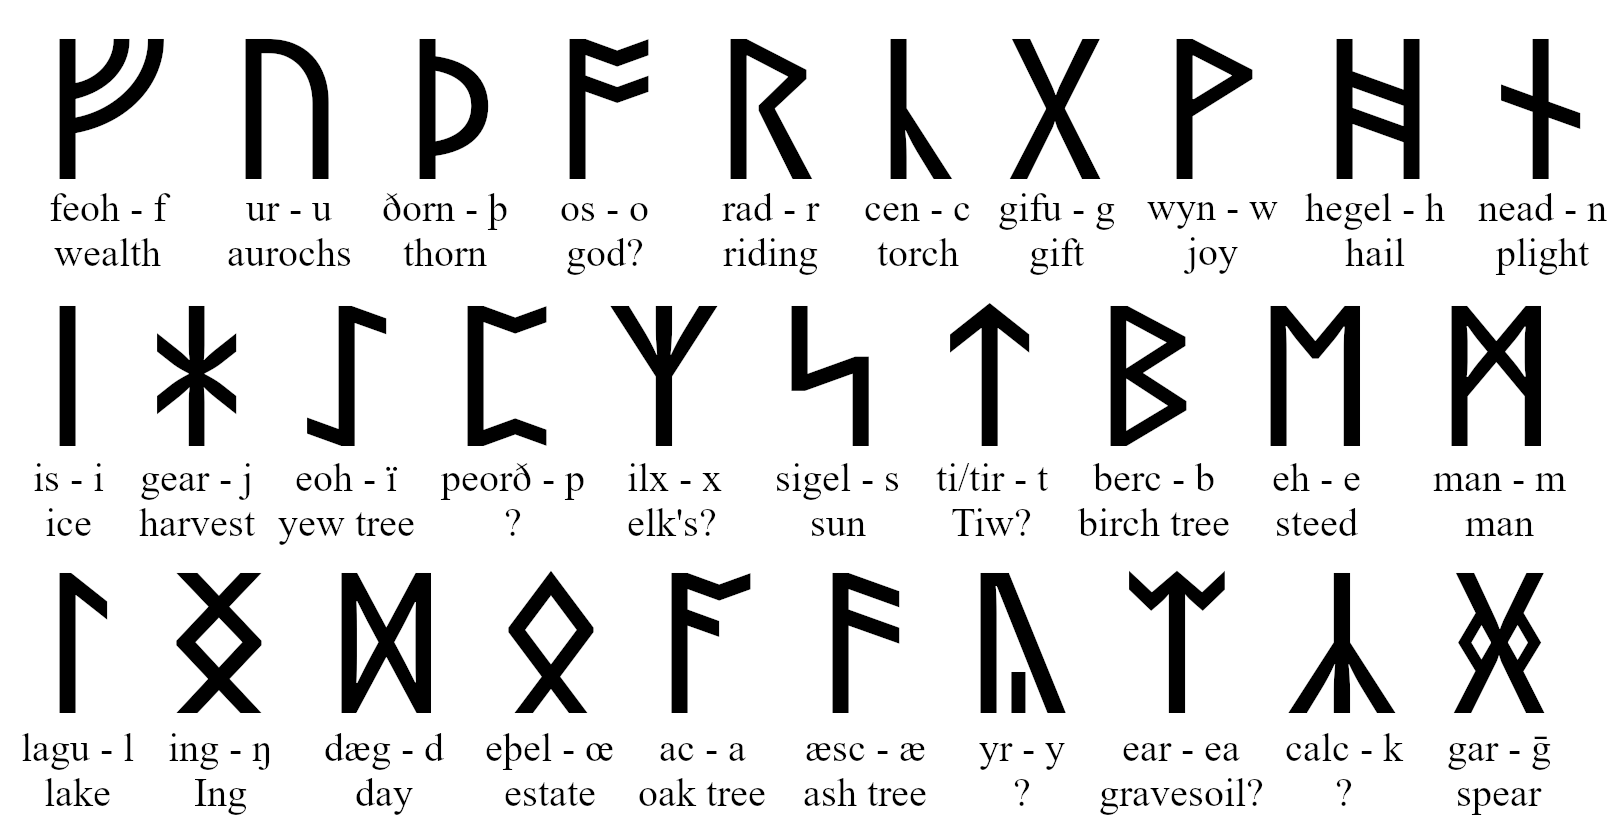
\includegraphics[width=0.8\textwidth]{figures/Futhorc_Rune_Chart.png}
\caption{The Anglo-Saxon futhorc (runic alphabet). Each rune is shown with its name, transliteration, and meaning. Source: By Blodcyning - Own work, CC BY-SA 4.0, \url{https://commons.wikimedia.org/w/index.php?curid=76035366}}
\label{fig:futhorc}
\end{figure}

Figure \ref{fig:futhorc} shows the Anglo-Saxon futhorc. Each rune represented a phoneme and had a name, often related to its shape or cultural significance. For example, the first rune, \textit{feoh} ⟨ᚠ⟩, meant `wealth' and represented /f/. 

The futhorc included runes for sounds not found in the Latin alphabet. Of particular interest is ⟨þ⟩, which represented the ``th sounds'' in Old English, as in \textit{thorn}, which was its name. It appears in the third position of the futhorc.

Runic writing served various purposes, from short inscriptions on objects to longer texts carved in wood or stone. While often associated with epigraphic uses, runes were also employed in manuscript writing before the widespread adoption of the Roman alphabet.

The Roman alphabet arrived in Britain with Christian missionaries in the late 6th century, most famously with Augustine's mission in 597 CE. But it didn't immediately replace the runic system. Instead, the two writing systems coexisted for several centuries, with the Roman alphabet gradually becoming dominant.

As the Anglo-Saxons adopted the Roman alphabet to write Old English, they faced a challenge: the Latin alphabet lacked symbols for some Old English sounds. To solve this, they repurposed some Latin letters, created new ones, and even borrowed from their runic heritage:

\begin{enumerate}[noitemsep]
    \item They created the letter ⟨æ⟩ (ash) to represent a vowel sound between /a/ and /e/.

    \item They used ⟨þ⟩ from the futhorc for the unvoiced /θ/ and introduced ⟨ð⟩ (eth) for voiced /ð/ (as in \textit{though)}.

    \item They used the runic wynn ⟨ƿ⟩ for the /w/ sound, before eventually replacing it with the double-u (⟨uu⟩, which became ⟨w⟩).

    \item The reason the double-u looks like two ⟨v⟩s instead of two ⟨u⟩s is that initially the vowel was written with the sharp shape ⟨v⟩ and the consonant as the rounded ⟨u⟩. While they switched placed in Middle English, the ``sharp u'' continued to be used for ⟨w⟩.
\end{enumerate}

Here's an example from the 8th century poem ``Cædmon's Hymn'', showing Old English written in the adapted Roman alphabet:

\begin{quote}
Nu sculon herigean heofonrices weard,\\
meotodes meahte and his modgeþanc,\\
weorc wuldorfæder, swa he wundra gehwæs,\\
ece drihten, or onstealde.
\end{quote}

\begin{quote}
    Now we must praise the Guardian of heaven,\\
    the Creator's might and His mind's plan,\\
    the work of the Glory-Father, as He for each wonder,\\
    eternal Lord, established the beginning.
\end{quote}

Notice the use of ⟨þ⟩ in \textit{modgeþanc} and ⟨æ⟩ in \textit{fæder} (father) and \textit{wæs} (was). This text shows how the Anglo-Saxons had adapted the Roman alphabet to their language while retaining some elements inspired by their runic heritage.

So, the transition to the Roman alphabet was a gradual process of adaptation rather than a simple replacement. It reflects the blending of Anglo-Saxon and Latin-based Christian cultures in early medieval England, a process that would profoundly shape the development of the English language and its writing system.

\subsection{The Norman Conquest and the Great Vowel Shift}\label{sec:great-vowel-shift}

The Norman Conquest of 1066 brought profound changes. French became the language of the nobility, while English continued among the common people. When English re-emerged as a written language in the 14th century, it had absorbed a wealth of French vocabulary~-- and French spelling conventions.

For instance, the Old English ⟨cwen⟩ became ⟨queen⟩, adopting the French ⟨qu⟩ for the /kw/ sound. The Old English ⟨scip⟩ became ⟨ship⟩, using ⟨sh⟩ to represent /ʃ/, a convention borrowed from French scribes.

Around the same time, English pronunciation was undergoing a major change known as the Great Vowel Shift. Over a period of several centuries, the pronunciation of most long vowels shifted upwards in the mouth, with the highest vowels becoming diphthongs. Figure \ref{fig:great-vowel-shift} illustrates these changes:

\begin{itemize}[noitemsep]
    \item \textit{bite}: Middle English /biː.tə/ became Modern English /baɪt/
    \item \textit{beet} Middle English /beːt/ shifted to Modern English /biːt/
    \item \textit{beat}: Middle English /bɛːt/ moved to Modern English /biːt/
    \item \textit{bate}: Middle English /baː.tə/ shifted to Modern English /beɪt/
\end{itemize}

\begin{figure}[h]
    \centering
    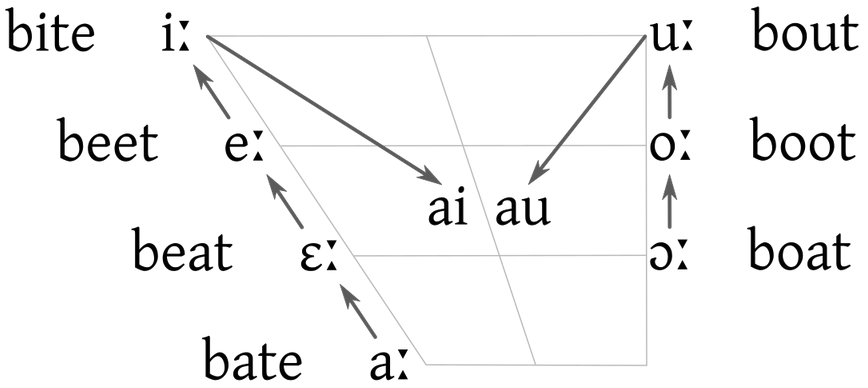
\includegraphics[width=0.8\textwidth]{figures/Great_Vowel_Shift2c.png}
    \caption{The Great Vowel Shift in English. This diagram shows the changes in pronunciation of long vowels from Middle English to Modern English. Source: Goran tek-en, CC BY-SA 4.0 \url{https://creativecommons.org/licenses/by-sa/4.0}, via Wikimedia Commons}
    \label{fig:great-vowel-shift}
\end{figure}

The Great Vowel Shift explains many seeming irregularities in English spelling and pronunciation. Here's an illustrative example:

\textit{Please} and \textit{pleasant}:
\begin{itemize}[noitemsep]
  \item In Middle English, \textit{please} was pronounced /plɛːzə/ (with a long /ɛː/), and \textit{pleasant} was /plɛzənt/ (with a short /ɛ/). The ⟨pleas⟩ sounded the same, other than that the ⟨ea⟩ of \textit{please} was drawn out longer than was that of \textit{pleasant}.
  \item The long /ɛː/ in \textit{please} shifted~-- along with the other long vowels. It went through /eː/ to become /i/, giving us Modern English /pliz/.
  \item The short /ɛ/ in \textit{pleasant} was unaffected, being short, resulting in Modern English /plɛzənt/.
  \item This shift caused these words that once shared their first vowel to diverge in pronunciation.
\end{itemize}

This example demonstrates how the Great Vowel Shift created discrepancies between spelling and pronunciation, and between related words. It also shows how other factors, such as vowel length, interacted with the shift to shape Modern English pronunciation.

The ``silent e'' in Modern English spelling is another fossil left by the Great Vowel Shift. Back in Middle English, that ⟨e⟩ wasn't silent at all~-- it was pronounced as a schwa /ə/ (like the last vowel in \textit{sofa}). So ⟨name⟩ wasn't just /neɪm/, but /naːmə/.

When the Great Vowel Shift hit, it mainly affected long vowels. Here's what happened: The vowel in the first syllable got longer and changed quality: /aː/ shifted to /eː/ and eventually to /eɪ/. That final /ə/ gradually disappeared, and the /m/ attached itself to the first syllable.

But the spelling stuck around, like a vestigial tail. Now that ⟨e⟩ serves a new purpose: it's a signal that the preceding vowel is ``long''. But remember, today's ``long'' vowels aren't really prolonged; they're just diphthongs in many cases.

\begin{itemize}[noitemsep]
    \item ⟨bite⟩: Middle English /biː.tə/ → Modern English /baɪt/
    \item ⟨name⟩: Middle English /naː.mə/ → Modern English /neɪm/
    \item ⟨rose⟩: Middle English /rɔː.zə/ → Modern English /roʊz/
\end{itemize}

In each case, that final ⟨e⟩ used to be its own syllable. Now it's just hanging out, reminding us of a pronunciation long gone.

This ``silent e'' rule isn't foolproof~-- English loves its exceptions. But it's a handy fossil, showing us how the Great Vowel Shift left its mark not just on our pronunciation, but on our spelling too.

\subsection{The impact of printing and classical learning}

The printing press arrived in England in 1476, brought by William Caxton. This new technology changed how books were made and, over time, influenced English spelling.

Before the printing press, scribes wrote books by hand, often spelling words based on their local dialects. Caxton and other early printers faced a challenge: which spellings to use? They made choices that would influence English orthography for centuries.

Caxton often chose spellings from his native Kent dialect. For example, he preferred ⟨gh⟩ in words like ⟨right⟩ over the northern ⟨rigt⟩. At the same time, a renewed interest in classical learning led printers and scholars to modify spellings to reflect (often erroneously) Latin or Greek origins:

   \begin{itemize}[noitemsep]
     \item The silent ⟨b⟩ in ⟨doubt⟩ and ⟨debt⟩ was added to echo Latin \textit{dubitare} and \textit{debitum}.
     \item The ⟨s⟩ in ⟨island⟩ was added due to a mistaken connection with Latin \textit{insula}, though the word actually comes from Old English \textit{igland}.
   \end{itemize}

These printed spellings spread as books became more common, but standardization was a gradual process. Even in Shakespeare's time, a century after Caxton, spelling remained quite flexible.

The printing press thus set in motion a long process of change. It didn't create a uniform spelling system overnight, but it did provide a mechanism for certain spellings to become more widespread and eventually standard.

\subsection{Dictionaries and standardization}

You might think dictionaries have been around forever, recording the ``correct'' spellings of words. But they're a relatively recent invention. The first English dictionary, Robert Cawdrey's \textit{A Table Alphabeticall}, didn't appear until 1604. And it was a far cry from the hefty tomes we know today. Cawdrey's book listed just 2,543 words, mainly those he thought would be unfamiliar to the average reader.

For centuries after Cawdrey, English spelling remained a bit of a free-for-all. Even great writers like Shakespeare weren't consistent. The Bard spelled his own name several ways, including ⟨Shakespeare⟩, ⟨Shakespear⟩, and ⟨Shakspere⟩.

But as the idea that English could be a language of books and learning began to take hold, there was a concurrent push for standardization. In 1755, Samuel Johnson published his \textit{A Dictionary of the English Language}. It was a massive undertaking, with 42,773 entries. Johnson didn't just list words; he included quotations showing how they were used. He also made choices about spelling, helping to establish norms.

But Johnson's dictionary wasn't the final word. Across the Atlantic in the U.S.A., Noah Webster was working on an American dictionary. Published in 1828, Webster's \textit{An American Dictionary of the English Language} aimed to standardize American English spelling. He's the reason Americans write ⟨color⟩ while Brits write ⟨colour⟩.

Webster argued for spellings that reflected pronunciation. He succeeded with words like ⟨center⟩~-- instead of ⟨centre⟩~-- and ⟨defense⟩~-- instead of ⟨defence⟩. But some of his more radical ideas, like spelling ⟨women⟩ as ⟨wimmen⟩, didn't catch on.

These dictionaries played a crucial role in standardizing English spelling. They became authorities that people could turn to for the ``correct'' spelling. Schools started teaching these standardized spellings, and printing presses used them consistently. And today, that consistency is maintained through spell-check and other automatic tools.

But there's still variation. British and American English maintain their spelling differences. Spellings like ⟨realize⟩ and ⟨realise⟩ coexist. Some words have multiple accepted spellings even within the same variety of English. Is it ⟨judgement⟩ or ⟨judgment⟩? Both are accepted.

\section{From reading words to really reading}

It's worth acknowledging that the main point of reading is not decoding words but understanding texts. Be that as it may, once you're able to decode words well, then reading isn't all that much different from listening. In both cases, it's mainly language comprehension. This is called the ``Simple View of Reading'' and can be expressed as the formula:
\[
\text{Decoding}~D \times \text{Language Comprehension}~LC = \text{Reading Comprehension}~RC
\]

If you're reading this textbook, then you might be very close to $D=1$ and $LC=1$, where 1 is perfect. Since, $1\times1=1$, it means your reading comprehension is excellent. 

On the flip side, if you were to try to read Italian or Indonesian  your decoding might be 0.95, but your language comprehension would be basically zero~-- assuming you don't speak those languages or any of their close relations. And since anything multiplied by zero is zero, you'd understand almost nothing at all of what you'd read: $RC=0$. This is a situation known as \textsc{hyperlexia}. There are disabilities that can lead to hyperlexia in one's ``mother tongue'', but it's quite rare and not something language teachers typically encounter.

Much more common are dyslexia and other reading disabilities.

\subsection{Dyslexia and other reading disabilities}

Dyslexia and other reading disabilities are not as rare as you might think. Some experts say up to one in five people might have some degree of dyslexia. That's like having six dyslexic students in a class of 30 adult learners.

An illiterate adult~-- either because of lack of opportunity or because of a reading disability~-- might be more like $0.2\times1=0.2$. In other words, even though this person can understand language (near) perfectly, their reading is only as good as their decoding skill, which is to say very poor.

Finally, someone who has trouble both with decoding words and with general language comprehension may have a general reading disability. Or they may just be a beginning language learner.

The Simple View of Reading places each of these different cases in one of the four quadrants shown in Figure \ref{fig:simple-view-quadrants}.

\begin{figure}
    \centering
    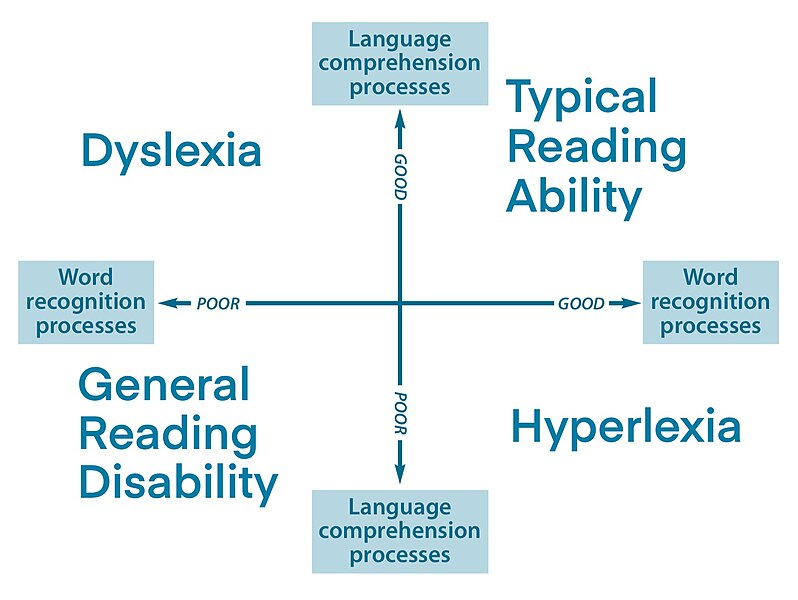
\includegraphics[width=0.8\linewidth]{figures/Simple_View_of_Reading_quadrant_visualisation.jpg}
    \caption{The four categories of readers predicted by the Simple View of Reading. By Smilingpolitely, \href{https://creativecommons.org/licenses/by-sa/4.0}{CC BY-SA 4.0}, via Wikimedia Commons}
    \label{fig:simple-view-quadrants}
\end{figure}

This overlap between language learning difficulties and reading disabilities can create significant challenges for English teachers. It becomes particularly difficult to distinguish between typical beginner-level struggles and potential reading disabilities in low-proficiency students. The situation is further complicated by several factors:

\begin{enumerate}[noitemsep]
    \item In many countries, awareness of dyslexia and other reading disabilities is limited, leading to underdiagnosis and lack of support.

    \item In the context of second language learning, reading difficulties are often attributed solely to the challenges of acquiring a new language.
    
    \item Most adult English learners with reading disabilities have likely never been diagnosed.
\end{enumerate}

As a result, English teachers need to be aware of the possibility of reading disabilities among their students, especially when learners show persistent difficulties that seem disproportionate to their overall language progress.

\bigskip

You've probably heard that dyslexia is about seeing letters backwards, mixing up ⟨b⟩ and ⟨d⟩, or reading ⟨form⟩ as ⟨from⟩. That's mostly a myth. Dyslexia is typically a phonological processing problem, a result of a brain struggling with the sounds of language \citep{lyon2003definition}. An adult with dyslexia might know exactly what a resume is, but struggle to identify each of the individual phonemes in /rɛzjumeɪ/. This makes it very hard to connect them to the individual letters ⟨r-e-s-u-m-e⟩.

Phonological processing difficulties offer one reason why it's so important to teach decoding skills explicitly. For many adults, especially those with dyslexia, these skills don't just develop naturally. They need systematic instruction and lots of practice. They might need extra help learning that ⟨ough⟩ can make different sounds in ⟨tough⟩, ⟨through⟩, ⟨though⟩, ⟨bough⟩ and ⟨cough⟩.

So where does this leave us? Sure, the ultimate goal of reading is understanding. But to get there, we've got to nail the basics. Decoding matters. And for some readers, it matters a whole lot more than for others.

\subsection{Teaching decoding}

When it comes to learning English, almost every interaction with the language is going to improve language comprehension. Even just having a conversation may be useful for lower-level students. Decoding, on the other hand, requires more focused attention. While it's true that some learners will pick up decoding skills naturally through exposure, many won't. This is especially true for adult learners who may have struggled with reading in their first language or who are coming from a language with a very different writing system.

Decoding isn't just about recognizing individual letters. It's about understanding how letters combine to represent sounds in English. Take the word ⟨thought⟩. A learner needs to recognize that ⟨th⟩ represents /θ/, ⟨ough⟩ represents /ɔ/, and ⟨t⟩ represents /t/. And that's a tricky word~-- there are plenty of others where ⟨ough⟩ represents different sounds entirely.

Two mistakes often crop up here. The first is when we work on decoding to the exclusion of other aspects of English. This can be very frustrating, especially if students are working on words they don't know. This has been derisively called ``teaching students to bark at print,'' and not entirely without reason. A somewhat related issue comes up  when students are already quite competent at decoding but teachers continue to put a lot of focus on decoding. Such a situation can be a frustrating waste of time, but fortunately I have rarely run into this.

The second mistake is to ignore decoding skills. There are various reasons they might be set aside. One is simply that working on these skills is rarely interesting or easy. In fact, it's often hard and boring for both the student(s) and the instructor. People quite reasonably want to get into the more meaningful (literally) activities. This is understandable but should be resisted.

A final reason is that many TESL programs don't address decoding skills. This means that the prospective teachers either aren't aware of decoding as an issue or don't know how to teach it. This chapter can't train you to teach decoding (though see Section \ref{sec:phonics}), but at least it should provide you with some awareness of the issue.

Decoding, like many things, is something that becomes easier with time and practice. At some point, it becomes automatic, you might even call it ballistic: once it has started, you can't stop it. You simply cannot look at a word on this page and NOT decode it. This level of automaticity is reached typically with some instruction on decoding and a lot of practice reading or being read to. Listening and reading at the same time can be particularly helpful.

\subsection{Teaching real reading}

At the same time that students are learning to decode, they should also be given lots of opportunities to listen, read, talk, and generally interact with language. The process of really reading is often cognitively indistinguishable from the process of listening. But there are a few distinctions that are worth pointing out.

One way that reading is easier is that, when you're reading, you're in charge. You can slow down, speed up, or go back. Imagine an adult learner comes across the word \textit{copacetic}. They can pause, sound out /kəʊpəsɛtɪk/, maybe even look it up. That kind of flexibility isn't available when listening to the radio, for example.

But reading presents its own challenges too. Written language often uses more complex words and longer sentences than spoken language. A business email might say, \textit{Please find attached the quarterly financial projections for your perusal,} a kind of language you'd rarely hear in the break room.

There's another big difference between reading and listening. When your colleague explains a new procedure, you're not just hearing words. You're seeing their gestures, where they're looking, and what they're holding. You're also hearing their tone of voice, and you can ask them to explain if something's not clear. At the same time, your colleague is able to see your expression and judge how well you're following.

But when you're reading a manual, it's just you and the words. The language lacks extra-linguistic context, and that can make reading more challenging than listening. But this is the kind of challenge that most adult learners of English will have already faced and overcome in another language.

Once they're up and reading in English, then, the challenge is achieving fluency, in both decoding and language comprehension. Fluency is the topic of Chapter \ref{ch:fluency}. For now, we turn our attention back to syntax, looking at questions and interrogatives.